% !TEX encoding = UTF-8 Unicode
% !TEX TS-program = lualatex
% !BIB TS-program = biber

%%%%%%%%%%%%%%%%%%%%%%%%%%%%%%%%%%%%%%%%%%%%%%%%%%%%%%%%%%%%%%%%%%%%%%%%%
%%%%% This version of toptesi-scudo-example. tex and its subsidiary %%%%%
%%%%% file are typeset with version 6.2.09 of the TOPtesi bundle.   %%%%%
%%%%%%%%%%%%%%%%%%%%%%%%%%%%%%%%%%%%%%%%%%%%%%%%%%%%%%%%%%%%%%%%%%%%%%%%%

%%%%%%% The above first line is used to auto-configure those LaTeX
%%%%%%% friendly editors, such as TeXShop, TeXworks, TeXstudio 
%%%%%%% so as to use the UTF-8 encoding for editing the source
%%%%%%% files and to save them.

%%%%%%% For the same editors the second line specifies which 
%%%%%%% typesetting engine is to be used when hitting the editor's
%%%%%%% button that launches the typesetting job.
%%%%%%% You can chose between pdflatex, lualatex or xelatex; in general
%%%%%%% it is better to avoid using xelatex and to prefer lualatex.



\documentclass[%
   corpo=12pt, % optional; default:= 10pt
   twoside, % recommended
   tipotesi=scudo,
   mybibliostyle, % only if biblio is typeset with a personal style
%  numerazioneromana, % not necessary in a real thesis
   ]{toptesi}
   
%%%%%%% If and only if you want to produce an archivable document
%%%%%%% according to the ISO regulation 19005:2005-1b add the
%%%%%%% following code after the statement \documentclass, and
%%%%%%% adapt its contents to your particular thesis.
%%%%%%% -----------------------------------------------------------
%%%%%%% This environment should be here, after the class has been
%%%%%%% specified and before the pdfx package is loaded.
%%%%%%% Previous versions of TOPtesi required the environment to be
%%%%%%% before the \documentclass statement; it is possible to maintain
%%%%%%% this habit for backwards compatibility, but by doing so, you
%%%%%%% give up the facility of overwriting a previous version of
%%%%%%% the .xmpdata file when you modify its contents, and you have
%%%%%%% to delete any previous version in advance. If you set this
%%%%%%% environment after the \documentclass statement, it overwrites
%%%%%%% any previous version of the .xmpdata file and you don't need
%%%%%%% to remember to delete it in advance.
%%%%%%%
%%%%%%% Do not worry if some Warnings are output at \begin{document}
%%%%%%% time about certain options being already been used.

\begin{filecontents*}{\jobname.xmpdata}
\Author{Mario Rossi}
\Title{Writing Your Ph.D. Thesis with LaTeX}
\Subject{Doctoral dissertations in the SCUDO doctoral school}
\Keywords{PDF\sep
          PDF/A\sep
          ISO 19005\sep
          LaTeX\sep
          PhD Thesis\sep
          Engineering\sep
          SCUDO}
\Publisher{Politecnico di Torino}
\end{filecontents*}
%%%%%%% -----------------------------------------------------------
   
%%%% Use the following package if and only if you want to produce
%%%% an archivable document according to standard PDF/A-1b
%%%% No need to load package imakeidx, because it has already been
%%%% loaded by the specific module toptesi-scudo.
\usepackage[a-1b]{pdfx}
\usepackage[linesnumbered,ruled,norelsize]{algorithm2e}
%%%%%% Read the English documentation of TOPtesi in order to check
%%%%%% the special attention needed to produce ISO compliant
%%%%%% archivable files
%%%%

\ifPDFTeX
    \usepackage[utf8]{inputenc}% 
    \usepackage[T1]{fontenc}
\fi

\errorcontextlines=9% more information on the console in case of errors

%%%% Specify fonts here; chose one among these fonts by leaving just
%%%% one line without initial comment character.
%%%% With LuaLaTeX or XeLaTeX don't change fonts
\ifPDFTeX % using pdflatex
    \usepackage{lmodern} % Default
    %\usepackage{newtxtext,newtxmath}% Times eXtended for text and math
    %\usepackage{fourier}% Utopia, Helvetica and "monospace = ?"

\else % using lualatex (or xelatex)
% Here we use the Libertinus serif, sans serif, monospaced and math fonts;
% they are alla available with a complete up-to-date TeXLive installation.
% Without specifying any OpenType font, the Latin Modern OpenType ones are
% used by default; try commenting the setting for Libertinus Mono, run with
% LuaLaTeX and see what happens; you might prefer to keep the comment sign
% in this line.
    \usepackage{fontspec}
    \defaultfontfeatures{Ligatures=TeX}
    \setmainfont{Libertinus Serif}
    \setsansfont{Libertinus Sans}
    \setmonofont{Libertinus Mono}[Scale=MatchLowercase]
    \usepackage{unicode-math}% add special math stile option here
                             % for example [style=ISO]
% define one math font 
    \setmathfont{Libertinus Math}%
\fi


\usepackage{kantlipsum,mwe} % to produce dummy text and dummy figures



\makeindex[intoc]% collect material to index

%%%%%%%%%%%%%%%%%%%%%%%%%%%%%%%%%%%%%%%%%%%%%%%%%%%%%%%%%%%%%%
% This conditional code is an example of using a different bibliography
% style from the one predefined by the class.
% The usage of the conditional code (also with a different contents) is
% discouraged, because the predefined numbered bibliography style is the
% one generally used in scientific publications.
% Even if discouraged, it is not forbidden.
\ifmybibstyle 
  \usepackage[autostyle]{csquotes} % necessary for biblatex
  \usepackage[backend=biber,
              style=philosophy-classic,
              scauthors=all,
              sorting=nyt,
              natbib]{biblatex} % LaTeX specific bibliography handler
\fi 
\addbibresource{\jobname.bib}% bibliographic data base(s)
% It is recommended to name a single or the primary .bib file with the same
% name as the thesis master file: the macro \jobname contains that name.
% It is possible lo use a comma separated list of bibliographical databases
% but extreme care must be paid to the fact that all .bib files have
% actually different names, and that the citations key are really distinct
% among alla databases, not simply within a single database.
%%%%%%%%%%%%%%%%%%%%%%%%%%%%%%%%%%%%%%%%%%%%%%%%%%%%%%%%%%%%%%
% The following is to be loaded as the end of the preamble if one wants
% to use hyperlinks and/or urls to be typed within the thesis,
% except that after loading hyperref very few commands may be
% issued. One is the \includeonly command with its list of files;
% other packages may be loaded after hyperref, only if their
% documentation says so; some of these critical packages, but they are
% not the only ones, involve Right to Left languages or other
% oriental languages.
%
% Distinguish the hyperref call from the hyperref setup so as
% to avoid option clashes with other packages that may invoke 
% hyperref with different options.

\unless\ifcsname ver@hyperref.sty\endcsname\usepackage{hyperref}\fi
\hypersetup{%
    pdfpagemode={UseOutlines},
    bookmarksopen,
    pdfstartview={FitH},
    colorlinks,
    linkcolor={blue},
    citecolor={blue},
    urlcolor={blue}
  }
%%%%%%%%%%%%%%%%%%%%%%%%%%%%%%%%%%%%%%%%%%%%%%%%%%%%%%%%%%%%%%

%%%% The \includeonly argument should preferably be written with
%%%% one file name per line, so that by commenting or uncommenting
%%%% some lines a selective compilation may be executed.
\includeonly{%
Chapter1/1_introduction,%
Chapter2/2_datacollection,%
%Chapter3/chapter3,%
%Appendix1/appendix1,
%Appendix2/appendix2,%
}
%%%%%%%%%%%%%%%%%%%%%%%%%%%%%%%%%%%%%%%%%%%%%%%%%%%%%%%%%%%%%%
\newcommand{\tool}{\textit{UMAP}\xspace}
\newcommand{\MGM}[1]{#1}
\newcommand{\removelatexerror}{\let\@latex@error\@gobble}

\ifPDFTeX \usepackage{indentfirst}\fi
\raggedbottom

\begin{document}

% The contents of this ThesisTitlePage environment may be written
% in a configuration file named exactly the same as the thesis main
% file, but with extension .cfg. If similar commands with different
% data are written within this environment, such data prevail on
% those read from the configuration file.
\begin{ThesisTitlePage}
% Use the optional command to set a different School logo
% Its is possible to used this command several times; each time
% a new different  Institution logo  may be added. In general
% just the ScuDo logo is sufficient; for dissertations made in
% cooperation with the University of Turin, its logo may be added
% with a second instance of the \PhGschoolLog statement. With
% dissertations supported by the INRiM, this institution logo may
% be added. Such logos (in PDF format) may be obtained from the
% ScuDo web server.
\PhDschoolLogo{TiTDocScCropped}% Fake logo for this example
%\PhDschoolLogo{Logo-ScuDo-blu} % just the ScuDo logo
%\PhDschoolLogo{Logo-ScuDo-blu,Logo-INRIM} %for dissertations made in cooperation with INRIM
%\PhDschoolLogo{Logo-ScuDo-blu,Logo-INFN} %for dissertations made in cooperation with INFN
%\PhDschoolLogo{Logo-ScuDo-blu,Logo-UniTo} %for dissertations made in cooperation with the University of Turin
% Doctorate course name; mandatory
\ProgramName{Energy Engineering}
% Cycle ordinal number; optional.
% You can write 29.th, or 29\ap{th}, or 29\textsuperscript{th}, or ...
\CycleNumber{29.th}
% PhD candidate name; mandatory
\author{Mario Rossi}
% Dissertation title; mandatory
\title{Writing your Doctoral~Thesis\\with \LaTeX}
% Dissertation subtitle: optional.
% It might be useful only if the actual full title is too long.
\subtitle{This document is an example of what you can do\\with~the~TOPtesi class}
% The supervisor(s) label; optional; default value "Supervisor:".
% You can change it to plural as in this example, where the colon has
% been eliminated.
%\NSupervisor{Supervisor}{Supervisors}
%
% The SupervisorNumber may contain a value such as 0, 1, or any
% number higher than 1. If 0 is specified, no label is typeset
% over the supervisor(s) list; if 1 is specified then the singular
% form is used: if any value higher than 1 is specified, the plural
% form is used.
\SupervisorNumber{2}
% List of supervisors with academic title, name(s), surname(s),
% and function; mandatory
\SupervisorList{%
    Prof.~A.B., Supervisor\\
    Prof.~C.D. Co-supervisor}
% Name of the examining committee: optional. 
% Default value "Doctoral Examination Committee"
%\Nexaminationcommittee{Doctoral examination committee}
% List of the  examining committee members: mandatory if the above label
% is not empty.
\ExaminerList{%
Prof.~A.B., Referee, University of \dots\\
Prof.~C.D., Referee, University of \dots\\
Prof.~E.F., University of \dots\\
Prof.~G.H., University of \dots\\
Prof.~I.J., University of \dots}
% Name of the institution where the examination takes place; optional.
% Default value: "Politecnico di Torino"
%\Nlocation{Politecnico di Torino}
% Examination date: mandatory, although the way to write it is free.
\ExaminationDate{February 29, 2123}
% Disclaimer with signature; optional. Default text as
% in the following lines. 
\Disclaimer{%
\noindent I hereby declare that, the contents and organisation of this dissertation constitute my own original work and does not compromise in any way the rights of third parties, including those relating to the security of personal data.	
}
%\Signature{%
%\begin{flushright}
%\parbox{0.5\textwidth}{\centering
%\dotfill\\
%Mario Rossi\\
%Turin, February 29, 2123
%}
%\end{flushright}}
\end{ThesisTitlePage}
%%%%%%%%%%%%%%%% Everything else necessary in the thesis title
%%%%%%%%%%%%%%%% page and in the copyright page is supplied by
%%%%%%%%%%%%%%%% the default values.
%%%%%%%%%%%%%%%% If you enter an explicit disclaimer, you can
%%%%%%%%%%%%%%%% typeset other material before the disclaimer
%%%%%%%%%%%%%%%% formula; use the necessary spacing on order
%%%%%%%%%%%%%%%% to separate the formula from other text. 
%%%%%%%%%%%%%%%% 
%%%%%%%%%%%%%%%% For example you might want to write the formal
%%%%%%%%%%%%%%%% statement for a particular licence, provided the 
%%%%%%%%%%%%%%%% licence allows Open access; not necessarily all uses
%%%%%%%%%%%%%%%% of the thesis should be allowed, but the minimum
%%%%%%%%%%%%%%%% is the reading access.

%%%%%%%%%%%%%%%% The next two lines are metadata for a normal PDF file.
%%%%%%%%%%%%%%%% For ISO archivable PDF/A-1b metadata, they must
%%%%%%%%%%%%%%%% be entered only in the form used in the file
%%%%%%%%%%%%%%%% named in the filecontents* environment as shown
%%%%%%%%%%%%%%%% at the beginning of this file.

%\subject{How to typeset a doctoral thesis suitable for defence in almost any country and university.}
%\keywords{{pdfLaTeX} {LuaLaTeX} {XeLaTeX} {PhD doctoral programs} {PhD dissertation} {Politecnico di Torino}} 

\summary%\sommario

This is where you write your abstract \dots\ (Maximum 4000 characters, i.e. maximum two pages in normal sized font, typeset with the thesis layout).

The abstract environment is also available, but  \texttt{\string\summary} is preferred because it generates an un-numbered chapter. The abstract environment is more suitable for articles and two column typesetting without a separate title page.

\emptypage %  it works even without the classica option
\acknowledgements% or \ringraziamenti

And I would like to acknowledge \dots

Acknowledgements are mandatory only when people outside the academic institution supported the development of the research that was performed in order to reach the conclusion of the doctorate program.

\begin{dedication}

\textit{I would like to dedicate this thesis to my loving parents} 

{\normalsize 
The dedication very seldom is a proper thing to do; in some countries it is very common, while in other countries it is done for imitation of other people habits. 

The sentence used above clearly is an example of something very common, but it is  useless. Of course we all love our beloved parents, but it is not necessary to ``engrave it in stone''.
\par}
\end{dedication}
%\end{dedica}

%%%%%%%%% If you want these two lists, uncomment the following line
%\tablespagetrue\figurespagetrue % 

%%%%%%%%% Table of contents and optionally the tables and figures lists
\allcontents

\mainmatter %all the above is front matter; here begins the main matter

% !TEX root = ../toptesi-scudo-example.tex
% !TEX encoding = UTF-8 Unicode
%***********************************************************************
%*********************************** First Chapter 
%***********************************************************************

\chapter{Introduction}  %Title of the First Chapter
\label{chap:1_introduction}
    \graphicspath{{Chapter1/}}


descrivo la storia i benefit e la storia del carsharing



% !TEX root = ../toptesi-scudo-example.tex
% !TEX encoding = UTF-8 Unicode
%***********************************************************************
%***********************************Second Chapter
%***********************************************************************

\chapter{Data acquisition}
\label{chap:2_dataset}
	\graphicspath{{Chapter2/}}

Car sharing is nowadays a popular means of transport in smart cities. In particular, the free-floating paradigm lets the customers look for available cars, book one, and then start and stop the rental at their will, within a specific area. This is done thanks to a smartphone app, which contacts a web-based backend to exchange information. In this paper we present \tool, a platform to harvest the data freely made available on the web by these backends and to extract driving habits in cities.

We design \tool with two specific purposes. Firsty \tool fetches data from car sharing platforms in real time. Secondly, it processes the data to extract advanced information about driving patterns and user's habits. To extract information, \tool augments the data available from the car sharing platforms with mapping and direction information fetched from other web platforms. This information is stored in a data lake where historical series are built, and later analyzed using analytics modules easy to design and customize. 

We prove the flexibility of \tool by presenting a case of study for the city of Turin. We collect car sharing usage data for over 50 days to  characterize both the temporal and spatial properties of rentals, and to characterize customers' habits in using the service, which we contrast with public transportation  alternatives. Results provide insights about the driving style and needs, which are useful for smart city planners, and prove the feasibility of our approach.


\section{Introduction}
\label{sec:intro}

Mobility is one of the challenges to solve in our society and in cities, where eco-sustainability is becoming more and more important. 
Regulators and policy makers are positively looking into ``smart'' approaches to improve the current status of their urban network.  The ability to collect data, is the first step to take informed decisions. Unfortunately, getting information about mobility patterns and human driving habits is not easy because of both technical challenges and privacy issues.

To this extent, in this paper we investigate the possibility of harvesting data openly exposed on the Web to obtain information about mobility habits in cities, and make it available to the players by using a smart-platform. We focus on car sharing platforms and mapping and direction services.
%
%For many years the usage of a private car for transportation was the most important solution. Nowadays this trend seems to decrease, especially among young adults for who owning a private car look to be less important. This change to alternative mobility services favorites the growth of car sharing systems.
%
%The first known solution of such a system is the Selbstfahrergenossenschaft car  sharing program born in 1948 in Zurich without a former development of it. Only in the early 1970s saw a first system based on car sharing. However, only recently, with the growth of the sharing economy, the car sharing system accelerated its growth, making nowadays the car sharing widely used in different parts of the world. As a matter of fact, the importance of car sharing systems is demonstrated by the expansion in term of mermership number. According to~\cite{a,b} this growth exceeds 10\% per year either in North America and Germany.

%Among the key advantages of such a system, has been proved that it allows traffic and pollution reduction~\cite{}.

Car sharing refers to a model of car rental where customers rent a car for a short period of time, usually for a few hours or less. One of its most interesting systems is the so called \textit{Free-Floating Car Sharing (FFCS)} system. The peculiarity of this system is that customers can pick and drop the car wherever in a geo-fence area.
The most famous company is car2go which is present in 25 cities and 8 different countries, both in Europe and North America.

%, where customers rent a car via the web or a smartphone app
% In the station-based approach, users have to pick-up the car and release it in specific positions e.g., parkings spot reserved for this car. A first example of this system is the famous American \textit{Zipcar} service, which allows users to pick up the car in specific parking spots and then return the car in the same starting point. An alternative is the one-way solution, like  \textit{Autolib'} in Paris, an electrical car sharing system where users can rent a car in one station and return to a different one. The peer-to-peer solution is based on the idea that most private car are most of the time unused(90\% of the time according to some estimation~\cite{c,yltechrep}). In this model, cars are made available by private users. The company which manage this kind of service only takes care of providing the insurance and finding customers to rent the car. This system is quite new to the market and it is exploited by a few companies (the most important one is RelayRides, in the US).
%
To rent a car in a modern FFCS system, users check on their smartphone, or on the FFCS website, which cars are available in the neighborhood. Then, with a simple tap they can book a car, and start/end the rental. The FFCS app contacts a web-based backend server to fetch data about available cars, perform a booking, and accounting operations. Typically for this purpose web API are used, some of which are publicly documented~\cite{car2goAPI}. The same website and app offer information about the status of the car rental systems, and the same web API can be used to collect for free this information. In the past, this approach has been successfully used to obtain data for specific mobility studies -- see Sec.~\ref{sec:related} for more details.
In this work, we extend this idea and focus our attention on the acquisition and harvesting of this data by means of big data techniques to understand driving habits in a city. We take the city of Turin as a use case.

We design \tool, a platform to collect, process, augment, and store data in a data lake, where analytics let the analyst extract higher level information.
We build two crawlers to collect data from the \textit{car2go}  and \textit{Enjoy} platforms\footnote{\url{www.car2go.com}, \url{enjoy.eni.com}}, both present in Turin. Every minute, the crawler checks which cars are currently available. Every time a given car ``disappears'', it records the booking start time. The same booking ends when the crawler sees the car available back on the system. Some booking are actual ``rental'' in case the car moved from the prior parking position to another. Ingenuity must be used, e.g., to filter GPS fix issues (which may erroneously let a car ``move''), or to handle possible data collection issues (e.g., the website going down, or some cars undergoing in maintenance), or platform design (e.g., synchronous or asynchronous updates).

We let the crawler run to collect data for 52 days, from December 10th 2016 to January 31st 2017. We observed more than 104,000 \textit{bookings} and 86,000 \textit{rentals} for car2go, and 93,000 \textit{bookings} and 81,000 \textit{rentals} for Enjoy. 
%Then, we characterize how user booked or rented the car during such a period, discovering that during the business day FFCS systems are used much more with respect to the weekend. To have a better understating on what is the trend during these two parts of the week, we then characterize the rentals dividing the week in two and studying the trend per hour. We discovered that while during weekdays the system is quite unused during the night, during the weekend we observe twice as much rents with respect to during the week days, but with a reduction during the day especially in the morning. Then, we characterize for how long time users rent cars and how far they go. Interestingly, we first discovered that despite the different pattern between week days and weekend days, the time and the distance users use to use a car does not change. Secondly, we observed that users using car2go use the car also for longer trip due to the possibility to drop the car in the Airport parking lot. By analyzing the duration time in case of bookings without a rental instead, we observed that the higher probability is less then 5 minutes and then at 20 minutes for car2go and around 15 minutes for Enjoy. While the first can be explained by a system fault, the second cases depends on the maximum \textit{reservation time} i.e., the maximum time an user can reserve a car without paying any fee. 
With these datasets, we characterize the FFCS service utilization, in terms of bookings and rentals, with the aim to observe how people use these services, where they typically go, when, for how long the rental last, etc. Some observations are quite intuitive, e.g., people appear to be willing to use more the FFCS during weekdays and during peak-time. Counterintuitively, the rental duration and the driving distance show marginal changes over the day and weeks.

%When comparing the two platforms, we discover that car2go users \DG{sometimes} drive the car for longer trips than the Enjoy users. This is partially due to the possibility to reach the Airport with car2go but not for Enjoy. We also observe that the usage increases during weekend evenings. Both effects suggest a lack of public transport which may be considered by the municipality for improvements.

% By analyzing the duration time of all the bookings that do not describe a rental, we observe that the highest percentage of them have a duration equal or lower than 5 minutes,  other common values are 20 minutes for car2go and around 15 minutes for Enjoy. While the shortest interval can be explained by a system fault or a booking cancellation, the other durations time can be linked with the maximum \textit{reservation time} i.e., the maximum time an user can reserve a car without paying any fee. 

%\DG{MESSAGGIO HEATMAP TBD}

We complement the analysis by comparing the booking duration with the driving duration as suggested by Google Directions application, which we collect in real time for each rental. This allows us to find that 8.5\% of bookings last less than the Google driving time. 
This may be due to Google Directions overestimating the driving duration or, recalling that bookings  include the reservation time and the time to look for a parking spot, this may suggest that the time-based tariffs adopted by FFCS systems may encourage fast driving styles in the hope to reduce the rental cost.
We next compare the duration of the booking with the equivalent trip duration by public transport as returned again by Google Directions. We discover that rentals are 36\% shorter on average than public transport time, but  rentals start to be preferred when public transport time is higher than 10 minutes.

We presented our results to the Turin Transportation Authority, who found them to be extremely useful to understand people driving habits. We believe that \tool represents an important support tool for the investigation of car sharing users' habits. The scalable design of \tool allows the policy maker to collect data from many FFCS providers  and integrate it with other sources. This eases the analysis when taking in consideration trends and providers comparison. \tool allows the Transportation Authority to take informed decisions when planning public transport systems. This characteristic strengthens the potentiality of \tool for economical and sociological prediction and analysis. Our data-driven approach, combined with other more traditional tools like surveys, represents an interesting observation point for understanding potential services improvements, both for car sharing and public transport systems. We make available the source code of \tool for research purposes.\footnote{\url{github.com/MobilityPolito/}}

The reminder of this paper is structured as follows: Sec.~\ref{sec:related} discusses the related work. 
Sec.~\ref{sec:methodology} describes in details \tool data acquisition and analysis capabilities. Sec.~\ref{sec:results} presents our results: First, we characterize car2go and Enjoy car usage over time; second, how customers drive the cars and how they move in the city; finally, we show what are the users' driving habits and the correlation between booking time and the public transport time. Sec.~\ref{sec:conclu} concludes the paper.




\section{Data Acquisition}
\label{sec:2_3_data_acquisition}
\begin{figure}[h!]
\centering
%left top right top
 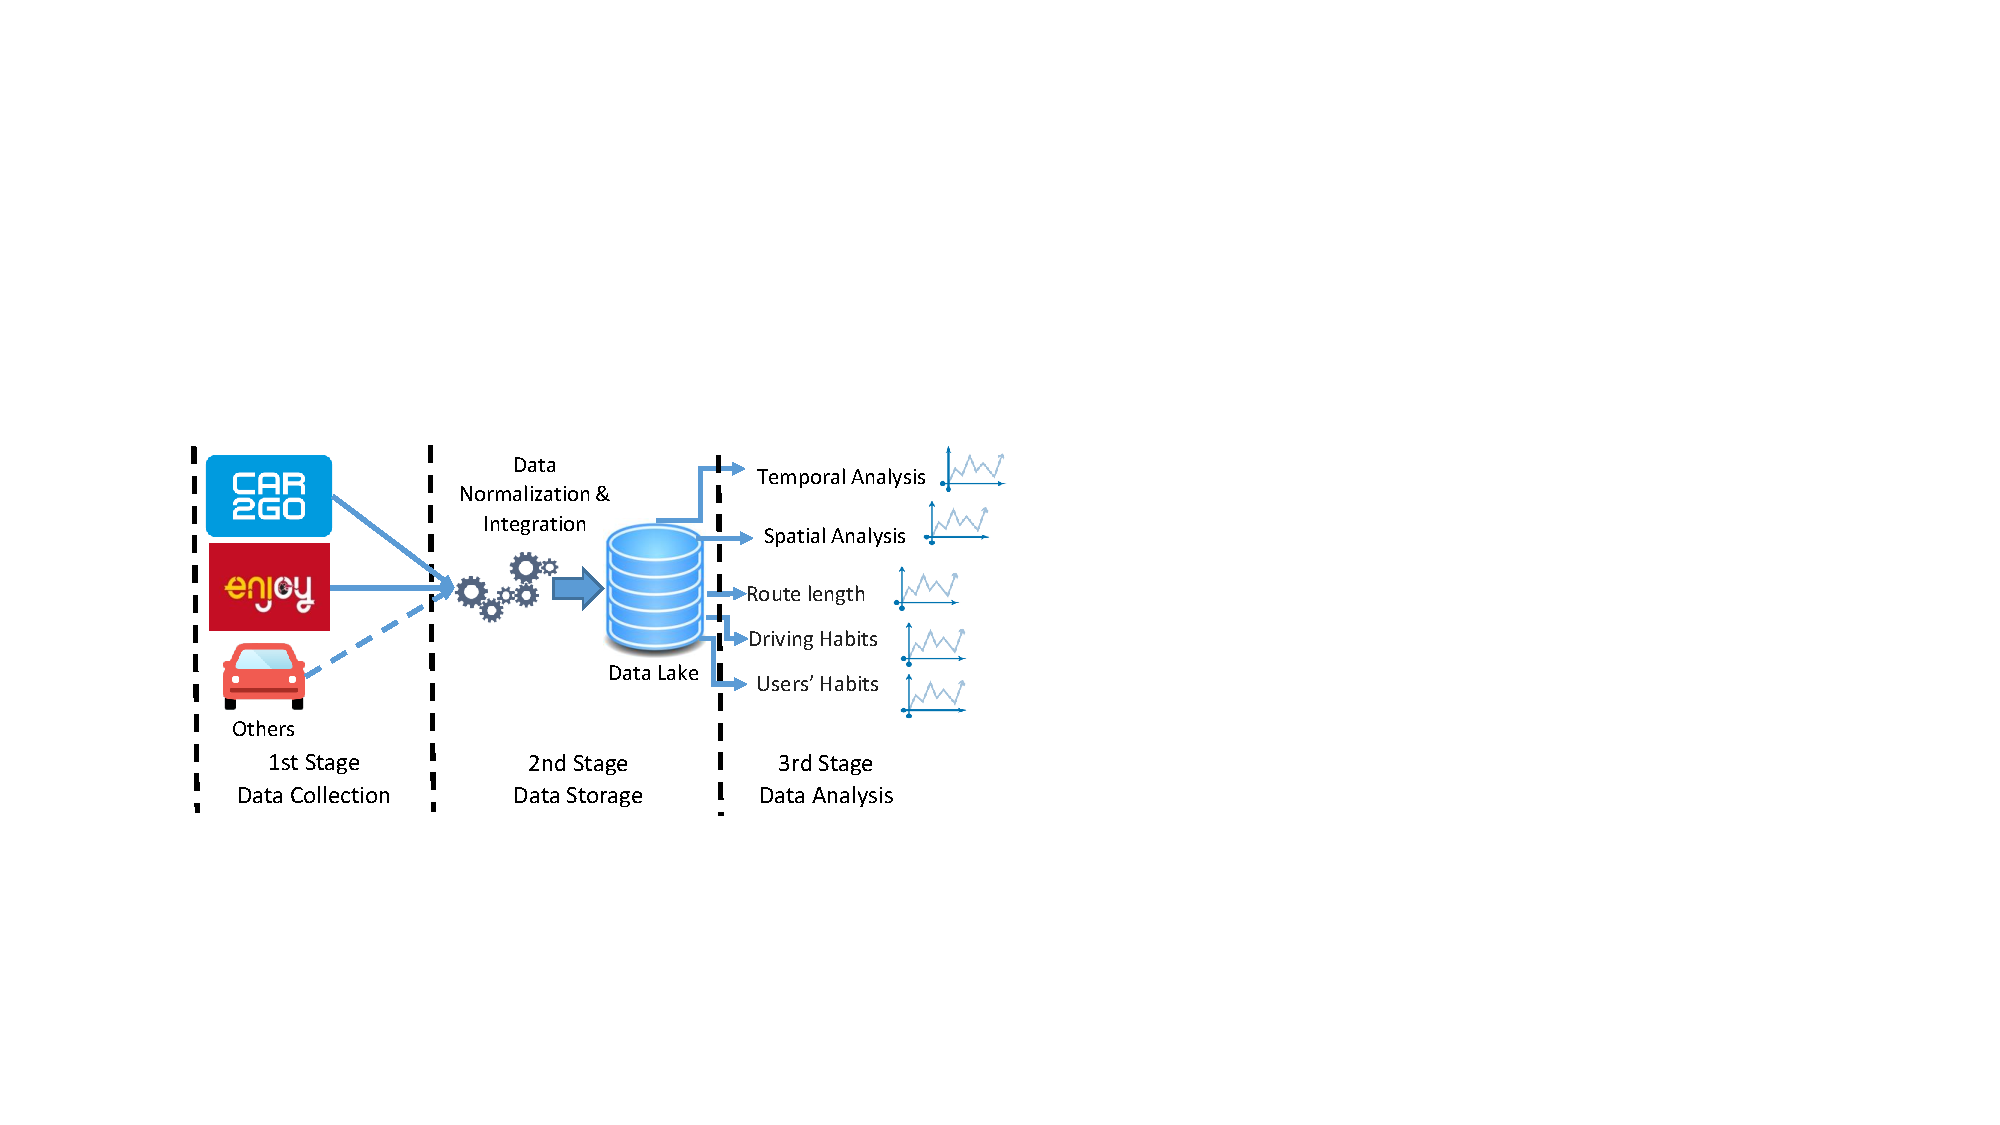
\includegraphics[trim=3cm 4.5cm 17cm 7.2cm,clip, width=0.95\columnwidth]{figures/framework_schema.pdf}
 \caption{\tool overview\label{fig:2_3_c2_framework}}
\end{figure}


In this section, I provide a description of \tool structure. Figure~\ref{fig:2_3_c2_framework} depicts the architecture of \tool, composed by a first module for the data acquisition, by a second module for data normalization and integration, and then a third  module for the data analysis.

The first module consists in the data acquisition from the car sharing platforms of interest. These typically expose information about cars' location when available for rental through a web-service approach. 

For this module I design two crawlers, one for the car2go and one for the Enjoy car sharing platforms. They retrieve, at each time instant, which cars are available in a given city.

While car2go offers public APIs~\cite{car2goAPI}, Enjoy does not provide to users such a service. For this reason I reverse engineer the Enjoy web portal. By leveraging the Chrome Developer Tools, I investigate the information exchanged with the Enjoy web portal while asking the list of available cars. Through this analysis, the software obtains both the URL used to request the list of available cars, and how fetch the data for a specific city.
Both system return the currently available cars using a JSON file.

Each time the system downloads a JSON, a \textit{snapshot} describing which cars are parked and ready for rental. Basically, the \textit{snapshot} is a list containing all cars and their attributes.

In a nutshell, a car is described by the car sharing web-service as an object annotated by several information, like plate, vehicle identification number (VIN), location, fuel level, model, etc. 
All the data represented in this object is useful for the customers e.g., to choose which car to rent.
This object is only present if the car is available, i.e., it is parked and free for a rental. Its state changes over time. In particular, a car disappears when a customer reserves and rents it, and then it reappears when the customer ends the rental (likely in a different location).


At each time $t$, the software gets the JSON snapshot $S$ listing the available cars. 
%We take a snapshot \textit{$S$} every minute to balance aggressiveness of the crawler, and time resolution. 
%At each time t, we obtain from each platform the JSON snapshot S detailing the available cars. 
The sampling period has been set to one minute, to balance aggressiveness of the crawler and a reasonable time resolution.
$S$ describes each available car with several fields, some of them being in common between the considered companies, but in general with different format.
For this study, I collect each car unique identifier and current geo-location indication.
These are obtained from the \textit{VIN} or \textit{plate} field, and the \textit{coordinates} field which describes the \textit{longitude} and the \textit{latitude} of the in-car GPS used to localize it when  parked.\footnote{The GPS coordinates are only available if a car is parked and available. There is no risk for users' privacy during rentals. In addition no user's identifier is exposed. Therefore data is totally anonymized as there is no means to know who booked a car.}
In addition to these fields, the car sharing JSON description may provide other information, e.g., the \textit{street address} corresponding to the coordinates, the \textit{fuel} level, the \textit{car interior status} the \textit{engine type}, etc. Since each platform uses its own data and format, I design a data integration step to have common names for fields containing the same information, if present.

\section{Data Normalization and Integration}
\label{sec:2_4_data_normalization}
In this second module I illustrates hoe \tool processes and consolidate each snapshot to obtain \emph{parking} and \emph{bookings} periods for each car. A \emph{parking} is time where the car is available for a user ride. On the other hand a \emph{bookings} is time elapsing two parking where the car is not tracked by the system. The intuition is to track the availability of each car on the car sharing platform, and rebuild the historic parking and booking periods over time: when a customer books a car, the latter ``disappears'' from the system. The framework records this event, with the initial time and position of a new booking. When the customer ends the booking, the car ``reappears'' in the system. The software records this event, with the final time and position of the booking. For the same car, a new parking period starts.

Harvested data is unstructured, and may grow large. Thus I leverage on \textit{MongoDB}, a NoSQL document-based database. A MongoDB database includes a set collections, i.e., groups of documents. Each document is a set of key-value pairs, organized in a JSON structure. The schema-less structure of MongoDB fits well in this work, because it can handle in the same collection documents defined with different key-value pairs. I decide to rely on such a system as I can easily manage the different field structures of providers, car2go and Enjoy in this use case. In addition, MongoDB offers a great integration with Python through the \textit{pymongo} module.

Four different collections compose the MongoDB data lake:  \textit{ActiveBookings}, \textit{ActiveParkings}, \textit{PermanentBookings}, and \textit{PermanentParkings}. 
\textit{ActiveBookings} and \textit{ActiveParkings} are collections used to store information about the current status of cars (currently booked or parked respectively). These are temporary structures that make it easier to query each car last observed status, and update it. These are also instrumentals for a real-time analysis of the system, e.g., to count how many cars are currently booked or available.
\textit{PermanentBookings} and \textit{PermanentParkings} collections store the history of past state of cars, for past bookings and parkings, respectively.

For the documents in the bookings collections I augment information by inserting also the expected route driving time, and the public transportation duration on the same origin-destination pair. These two piece of information are obtained through the Google Directions API using the initial and the final coordinates as indication of the path.

The most important fields in the \textit{ActiveBookings}, and the \textit{PermanentBookings} collections are:
\begin{itemize}
\setlength\itemsep{0.1em}
\item \textit{CarID}: the unique identifier of the car;
\item \textit{InitTime}: the initial time of the booking;
\item \textit{FinalTime}:  the final time of the booking;
\item \textit{InitCoords}:  the GPS coordinates of the booking star location, i.e., where the users picked up the car;
\item \textit{FinalCoords}:  the GPS coordinates of the parking location where the car was dropped at the end of the booking;
\item \textit{DrivingTime}: The duration of the trip, expressed in seconds, as estimated by Google Directions API, following the best path;
\item \textit{PublicTransportTime}: The duration is expressed as arrival time of the best public transport trip, as estimated by Google Directions API, minus the \textit{InitTime};
\end{itemize}

Instead, the \textit{ActiveParkings} and the \textit{PermanentParkings} collections are characterized by the following fields:
\begin{itemize}
\setlength\itemsep{0.1em}
\item \textit{CarID}: the unique identifier of the car
\item \textit{InitTime}: the initial time of the parking
\item \textit{FinalTime}:  the final time of the parking
\item \textit{Coordinates}: the GPS coordinates of the parking spot 
\end{itemize}

\begin{figure}[t!]
 \removelatexerror
 \scriptsize
  \begin{algorithm}[H]
   	\caption{Data acquisition at time $t$}
	\SetKwInOut{Input}{Input}\SetKwInOut{Output}{Output}
	\Input{$t$ - Current timestamp}
	\Input{$S$ - Available Cars (crawling result)}
	\BlankLine

	$AP$ = $Read(ActiveParkings)$ // Get previous available cars
	
	%\tcc{disappearedCars is a temporary list used to check the cars that %were visible, and that disappeared in the current crawling. In the %beginning the set will be equal to all the active Parkings}
	%$disappearedCars$ = $activeParkings$ \;
	\For(){$car_j$ in $S$}
	{
		\If{($car_j$  in $AP$)}
		{
			%\tcc{Update the parking information for that car with the %current timestamp}
			%$histogramNeighbours[final_time]$ = $current_timestamp$\;
			del $AP[car_j]$\;
		}
		\Else
		{
			$ActiveParkings.add(new~Parking(car_j,t))$\;		
			\If{($car_j$  in $ActiveBookings$)}
			{
				$FinalCoords = car_j[coords];$
				
				$ActiveBooking[car_j][FinalTime] = t$\;
				
				$InitCoords = ActiveBookings[car_j][InitCoords];$	
						
				\If{(checkCarMovement($InitCoords$,$FinalCoords$))}
				{
					$ActiveBooking[car_j][driving\_time]$ = $GoogleApi(driving,InitCoords,FinalCoords)$\;
					$ActiveBooking[car_j][PublicTranportTime]$ = $GoogleApi(public,InitCoords,FinalCoords)$\;
				}
				$MoveRow(car_j,ActiveBooking,PermanentBooking)$;
			}
			}
	}
	\For(){$car_j$ in $AP$}
	{
		$ActiveParking[car_j][FinalTime] = t$\;
		$MoveRow(car_j,ActiveParking,PermanentParking)$\;
		$ActiveBooking.add(new~Booking(car_j,t))$\;		
	}
  \end{algorithm}
   \caption{Pseudocode of the data acquisition algorithm}\label{pseudocodeCarInfoUpdate}
\end{figure}




I implemented an algorithm to extract booking and parking periods from snapshots, whose workflow is described in the pseudocode in Figure.~\ref{fig:3_2_c2_pseudocodeCarInfoUpdate}. Here I describe each  step.

I consider as inputs the snapshot $S$ and the current timestamp $t$.
Then I create a copy in the list $AP$ of parked cars observed in the previous snapshot (as stored in the $ActiveParkings$ collection) -- line 1. I need the $AP$ list to detect the cars that disappeared, i.e., have been booked at time $t$. This will be back explained later.

For each car $car_j$ in the current snapshot $S$, I check if the car is present in the $AP$ list. 
If so, it means that it did not change its status, i.e., it is still parked. Therefore, the car is removed from the $AP$ list, and nothing is changed -- lines 3-4.
Otherwise, either the car has been parked in this snapshot and the previous booking has finished, or the car is a new car added to the fleet. In both cases a new parking starts and I create a new document in the $ActiveParkings$ collection -- line 7. The \textit{new Parkings} function creates a new document, sets the $InitTime$ and $Coordinates$ keys as current timestamp and car GPS coordinates.
%with the current timestamp and the car GPS coordinates.

I next check if $car_j$ is present in the $ActiveBookings$ collection. If so, the car was booked until the previous snapshot and now it is back available. I thus finalize the previous booking and update its statistics. In particular, the tool sets the $FinalCoords$ and $FinalTime$ fields using the current car $coordinates$ and timestamp -- line 9-10. Next, I check if this booking includes an actual rental by checking if the initial position and final position differ -- line 11-12. Recall indeed that customers may simply book a car but not finalize the rental. Specifically, Enjoy (car2go) offers a grace period of 15 (20) minutes during which no charge is applied for a booking.

In case of an actual rental, I fetch the best path by i) car and ii) public transport from the  $InitPosition$ to the $FinalPosition$ of the rental. I leverage the Google Directions API for this -- line 13-14.\footnote{\url{https://enterprise.google.com/intl/it/maps/products/mapsapi.html}}
It is important to take into account that, while querying the public transportation time, the Google Directions API returns two pieces of information: how long the public transport takes to go from the initial to the final position, and the estimated arrival time. It is fundamental to use this second information because  it includes the time the user spends to reach the bus stop and wait for the bus. This is crucial, e.g., at night, when the first public transport solution may be available only several hours later.

After having processed all cars in the current snapshot, I iterate over the remaining cars in the $AP$ list. Those are the ones that were present in the previous snapshot, but not in the current, i.e., the ones the new bookings. Finally, the software adds to the previous parking period by setting the $FinalTime$ in the $ActiveParking$ collection -- line 21-22. At last, the tool creates a new booking via the \textit{new Booking} function -- line 23.


\begin{table}
	\setlength{\tabcolsep}{2.3pt}
	\centering
	\caption{Overview of car2go's data}
	\begin{tabular}{lcccc}
		\hline
		City &  City Size [$km^2$]\footnote{} & Population \footnotemark[\value{footnote}] &  Avg. Fleat & Bookings\\ 
		\hline
		\hline
		Columbus			  & 17 & 892k & 187 & 186k \\
		Florence 	  			& 34 & 372k & 220 & 333k \\
		Denver 		  			 & 36 & 727k & 312 & 348k \\
		Austin 		   			  & 31 & 964k & 315 & 377k \\
		Frankfurt 			   & 40 & 701k & 242 & 505k \\
		Toronto 				 & 49 & 3120k & 400 & 536k \\
		Amsterdam 			& 38 & 854k & 314 & 573k \\
		Montreal 				& 49 & 1704k & 429 & 606k \\
		New York City 	   & 77 & 8522k & 500 & 739k \\
		Turin 					    & 47 & 874k & 396 & 868k \\
		Munich 					 & 61 & 1464k & 478 & 916k \\
		Washington DC 	  & 64 & 705k & 563 & 919k \\
		Stuttgart 				 & 59 & 632k & 486 & 1001k \\
		Seattle 				   & 92 & 744k & 710 & 1134k \\
		Calgary 				  & 47 & 1239k & 552 & 1176k \\
		Rome 					  & 65 & 2837k & 582 & 1240k \\
		Rheinland 			   & 82 & 1688k & 648 & 1421k \\
		Vienna 					  & 72 & 1915k & 688 & 1702k \\
		Madrid 					 & 42 & 3233k & 424 & 2092k \\
		Milan 					   & 77 & 1396k & 776 & 2223k \\
		Hamburg 			  & 82 & 1833k & 812 & 2561k \\
		Vancouver 			 & 78 & 631k & 977 & 2701k \\
		Berlin 					  & 125 & 3769k & 1009 & 3091k \\
		%\\ \hline
		\hline
		\label{tab:2_3_datasummary}
	\end{tabular}
\end{table}
\footnotetext{\url{wikipedia.org}}
I let \tool scrape car2go's data  \mc{prendere le date}. In total it is possible to count about 27 million bookings spread in 23 cities. The table \ref{tab:2_3_datasummary} reports a brief resume of all the bookings, parkings present in the data lake. 

\mc{devo prendere le date anche di enjoy}



\section{Data Analysis}
The third and final stage is the data analysis phase in which analytics modules query the MongoDB and obtain statistics. I rely on the Python programming language with Pandas and the GeoPandas libraries to deal with the data, the city zone definitions, provided by transport engineers as a shapefile, a popular geospatial vector data format, and the Geographical Information Systems (GIS) for the spatial analyses. I choose Python as it offer a large number of  libraries that easily interact with the different technologies like GIS, maps and MongoDB. In particular the usage of GeoPandas allow me to easily perform geographic analysis and split the city in many areas (or zones) of any possible shapes. I present more detailed characterization in chapter \ref{chap:3_charact}.


\section{Conclusion}
In this chapter I described the software pipeline, named \tool I used to harvest and store data from real FFCS providers. 

The first stage explains the data structures and how I snapshots the system getting all the car ready for a ride. 

The seconds step illustrates the algorithm that compares consecutive snapshots detecting car status variation. Here I introduced the two fundamental car status I use to describe each car history: \textit{parkings} and \textit{bookings}. 

The third briefly opens several scenarios on the analyses of this data.



%\include{Chapter3/chapter3}
%% Numbered appendices remain in the main matter...
%\appendix
%\include{Appendix1/appendix1}
%\include{Appendix2/appendix2}

\backmatter% here begins the back matter
% ... otherwise a single appendix may stay here
%\include{References/biblio}

% Do not use this command if you did not prepare a nomenclature
% database by means of the suitable \nomenclature command and its
% arguments, as we did in chapter 2 of this example thesis.
\printnomencl

% In this example we use \nocite{*} in order to typeset the whole
% contents of the bibliographic database. Normally this is not
% necessary and it's better to let biber extract from the database
% only the cited works
%\nocite{*}


\printbibliography[heading=bibintoc]

% Do not use this command if you did not set the \makeindex switch
% in the preamble.

\printindex

\end{document}

